To dynamically compute the Smagorinsky
parameter in a local fashion, we follow the localized version of
the variational Germano identity (VGI) developed by
Tran \textit{et al.}~\cite{bib:tran2017b}.
In this procedure, Lagrangian averaging along fluid pathtubes is applied to make it robust and which maintains the localized nature of the VGI.
The dynamic local procedure and the associated assumptions and approximations are summarized in this section.

\subsection{Local Variational Germano Identity}
\label{sec:VGI}

The VGI involves comparing the variational form (including the model terms)
between different levels of the discretization.
In the localized version of the VGI, a set of nested spaces are constructed
by using a series of coarser second-level grids
along with the primary or original grid.
We refer to the primary grid as the $h$-grid and any grid in the
series of second-level grids as the $H$-level grid.
Each $H$-level grid is chosen such that it is associated with an
interior node in the primary grid.
This is done such that each $H$-grid is identical to
the $h$-grid except that the given node $k$ in the $h$-grid is coarsened or
removed resulting in a nested $H$-level grid for node $k$, which we refer to
as the $H_k$-grid.
Note that
each $H_k$-grid involves local coarsening around a given node $k$ while the remainder of the mesh remains the same.
This is
demonstrated in 1-D in Figure \ref{fig:vgi_grid},
where $\Omega^{H_k}$ is
the macro element in the $H_k$-grid corresponding to node
$k$ while $\Omega^{P_k}$ is the corresponding patch of elements
around node $k$ in the $h$-grid.
Note that $k = 1, 2, \ldots, n_{intr}$, where $n_{intr}$ is the number
of interior nodes in the $h$-grid. Therefore, there are $n_{intr}$
grids at the $H$ level, each of which is paired with the primary $h$-grid.
This results in the following spaces for each interior node,
$\bm{\mathcal{U}}^{H_k} \subset \bm{\mathcal{U}}^h \subset \bm{\mathcal{U}}$
and
$\bm{\mathcal{V}}^{H_k} \subset \bm{\mathcal{V}}^h \subset \bm{\mathcal{V}}$,
for the solution and weight functions, respectively.

\begin{figure}[H]
\centering
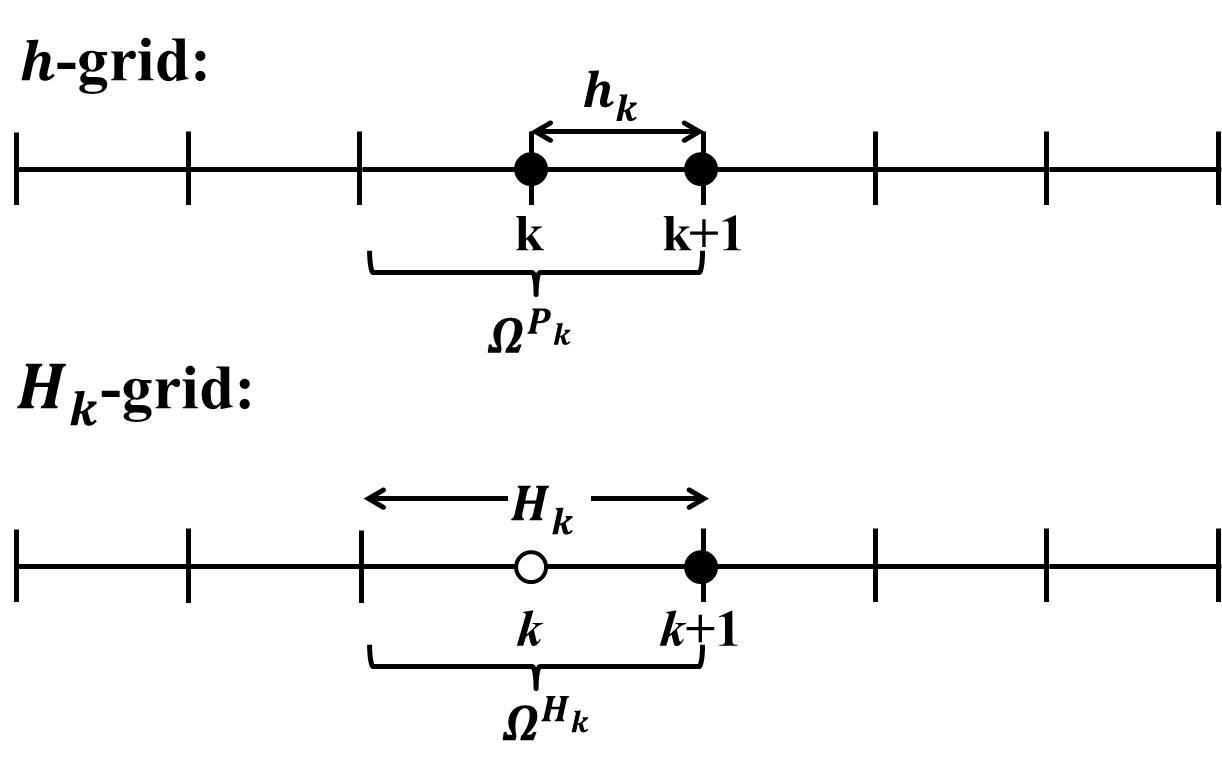
\includegraphics[width=0.45\textwidth]{figures/Setup/localization_grid.pdf}
\caption{1-D schematic of the $h$- and $H$-level grids for local VGI}
\label{fig:vgi_grid}
\end{figure}

The local VGI procedure then uses the
$H_k$-grids with the $h$-grid to compute the model
parameter at every node $k$ in the $h$-grid.
By setting $\bm{W}^h = \bm{W}^{H_k}$,
since $\bm{\mathcal{V}}^{H_k} \subset \bm{\mathcal{V}}^h \subset \bm{\mathcal{V}}$,
we get (for details see~\cite{bib:tran2017b})

\begin{equation}
\label{eq:vgil}
\begin{split}
 M_{comb}(\bm{W}^{H_k},\bm{U}^h; C^k_S, h_k) - M_{comb}(\bm{W}^{H_k},\bm{U}^{H_k}; C^k_S, {H_k})  = \\
  -(B(\bm{W}^{H_k},\bm{U}^h)- B(\bm{W}^{H_k},\bm{U}^{H_k}))
\end{split}
\end{equation}

We recognize that determining $\bm{U}^{H_k}$ for each interior node $k$ involves a grid-level
computation or projection (operations which involve looping over the elements of the $H_k$-grid). This is prohibitive and therefore, a surrogate is considered.
$\bm{U}^{H_k}$ is approximated within the macro element
using a volume-weighted average of $\bm{U}^h$ while outside
of the macro element the solution is assumed to be the same between the two grid levels.
This assumption further bypasses a grid-level computation. This assumption arises from the requirement on the variational multiscale (VMS) method to provide a localization at the element level and the desire to yield nodal exactness at element corners \cite{bib:hughes3}.
This leads to
$\bm{U}^{H_k} \approx \widetilde{\bm{U}}^{H_k}|_{\Omega^{H_k}} = \aHk(\bm{U}^h)$, where
$\aHk$ is the local averaging operator defined below.

\begin{equation}
\label{eq:avg}
\aHk (f^h) = \frac{1}{|\Omega^{P_k}|}\int\limits_{\Omega^h_e\in\Omega^{P_k}} f^h d\Omega^h_e
\end{equation}
\noindent where $|\Omega^{P_k}|$ is the volume of the local patch
and $\Omega^h_e$ indicates an element in the $h$-grid.

This choice is only feasible when the spatial derivatives exist on the weight function.
In addition, instead of using $\widetilde{\bm{U}}^{H_k}$ to compute $\bm{S}^{H_k}$ (strain-rate tensor), $\bm{S}^{H_k}$ is also approximated within the macro element as $\widetilde{\bm{S}}^{H_k}|_{\Omega^{H_k}} \approx \aHk(\bm{S}^h)$.
Furthermore, among all of the terms in Equation~\eqref{eq:vgil} 
not involving the unknown model parameter, the non-linear convective 
term is found to be dominating \cite{bib:tran2017b}. We note that this assumption holds 
exactly in a spectral setting where all the bilinear terms cancel out 
between the $H$- and $h$-level grids due to the $L_2$ orthogonality of 
spectral modes \cite{bib:oberai2005_2}. 
The local VGI simplifies to

\begin{equation}
	\label{eq:vgilb}
\begin{split}
M_{smag}(\bm{W}^{H_k},\bm{U}^{h}; C_S^k, h_k)_{\Omega^{P_k}} - M_{smag}(\bm{W}^{H_k},\widetilde{\bm{U}}^{H_k} ; C_S^k, H_k)_{\Omega^{H_k}} \approx\\
-(B_2(\bm{W}^{H_k},\bm{U}^{h})_{\Omega^{P_k}} - B_2(\bm{W}^{H_k},\widetilde{\bm{U}}^{H_k})_{\Omega^{H_k}} )
%-(B_2(\bm{W}^{H_k},\bm{U}^{h})_{\Omega^{P_k}} - B_2(\bm{W}^{H_k},\widetilde{\bm{U}}^{H_k})_{\Omega^{H_k}}) \approx \\
 %M_{smag}(\bm{W}^{H_k},\bm{U}^{h}; C_S^k, h_k)_{\Omega^{P_k}} - M_{smag}(&\bm{W}^{H_k},\widetilde{\bm{U}}^{H_k} ; C_S^k, H_k)_{\Omega^{H_k}}
\end{split}
\end{equation}

Now an appropriate choice for $\bm{W}^{H_k} \in \bm{\mathcal{V}}^{H_k}$ must be made. 
In a 1D setting, we select
$\bm{W}^{H_k}=[w^{H_k}_i,0]^T$ with $w^{H_k}_i$
such that it is linear along a spatial direction within the
macro element and is constant or flat outside.
Within the macro element, $w^{H_k}_i$ is selected such that

\begin{equation}
\label{eq:wij}
w^{H_k}_{i,j} = \frac{1}{|\Omega^{H_k}|}
\end{equation}

\noindent where $|\Omega^{H_k}|$ is the volume of the
element. 
% In Figure \ref{fig:vgilocal}, $w^{H_k}_i$ is shown in 1D (in the $x_j$ direction).
% \begin{figure}[H]
% \centering
% \includegraphics[width=0.75\textwidth]{figures/localization.jpg}
% \caption{A 1D schematic of $w^{H_k}_i$ for the local VGI procedure}
% \label{fig:vgilocal}
% \end{figure}
This choice of $\bm{W}^{H_k}$
is feasible in a multi-D setting and on an
unstructured mesh consisting elements of mixed topology,
however, a larger patch must be considered. An extra layer
of elements is needed around the macro element to attain a constant value
in the outside region. This extra layer acts as a buffer region.
This choice is made due to its ease of implementation.
For more details see~\cite{bib:tran2017b}.


\subsection{Local Variational Germano Identity Computation}
\label{sec:VGIComp}

At this point we drop the subscript $k$ in $H_k$ and $P_k$ and superscript
$k$ in $C_S^k$ for brevity and only use it when necessary.
The residual of the local VGI is defined as

\begin{equation}
\label{eq:vgilres}
\epsilon_{ij} = L_{ij} - 2 (C_S h)^2 M_{ij}
\end{equation}
\noindent where
\begin{equation}
\label{eq:lij}
L_{ij} = \left(\left(\frac{1}{|\Omega^H|}, u^h_i u^h_j\right)_{\Omega^P} - \left(\frac{1}{|\Omega^H|}, \widetilde{u}^H_i \widetilde{u}^H_j\right)_{\Omega^H} \right)
\end{equation}
\begin{equation}
\label{eq:mij}
M_{ij} = \left(\left(\frac{1}{|\Omega^H|}, |S^h| S^h_{ij}\right)_{\Omega^P} - \left(\frac{H}{h}\right)^2\left(\frac{1}{|\Omega^H|}, |\widetilde{S}^H| \widetilde{S}^H_{ij}\right)_{\Omega^H} \right)
\end{equation}

The least squares method is applied to determine the model parameter as follows
\begin{equation}
\label{eq:vgi_cs}
(C_S h)^2 = \frac{1}{2}\frac{L_{ij}M_{ij}}{M_{ij}M_{ij}}
\end{equation}

Since the local VGI procedure can lead to negative values
for $(C_S h)^2$, an averaging scheme is employed to avoid this issue.
Specifically, Lagrangian averaging 
is applied \cite{bib:meneveau96}.
To do so, two additional advection-relaxation scalar equations are solved.
These are shown in Equations~\eqref{eq:ILM} and~\eqref{eq:IMM}.
The scalars $I_{LM}$ and $I_{MM}$ in these equations are the
Lagrangian-averaged counterparts of
$L_{ij} M_{ij}$ and $M_{ij} M_{ij}$, respectively.

\begin{equation}
\label{eq:ILM}
  I_{LM,t} + (u_j - u^m_j) I_{LM,j} = \frac{1}{T} (L_{ij}M_{ij} - I_{LM})
\end{equation}

\begin{equation}
\label{eq:IMM}
  I_{MM,t}+ (u_j - u^m_j) I_{MM,j} = \frac{1}{T} (M_{ij}M_{ij} - I_{MM})
\end{equation}

\noindent where $T$ is the timescale over which averaging is applied.
Additionally, a local volume-weighted averaging
is also applied separately to the numerator and denominator
of Equation~\eqref{eq:vgi_cs} as follows

\begin{equation}
\label{eq:CS_LDS}
  (C_S h)^2 = \frac{1}{2}\frac{\aH(I_{LM})}{\aH(I_{MM})}
\end{equation}

\noindent where, as before, $\aH$ represents a local averaging operator.
This is equivalent to averaging over local pathtubes \cite{bib:tran2016,bib:tran2017b} and maintains the utility of the local VGI.

